\begin{frame}
  \begin{center}
    {\huge GloVe: Global Vectors for Word Representation
    } \\
    Pennington,Socher,Manning
  \end{center}
\end{frame}
%%%%%%%%%%%%%%%%%%%%%%%%%%%%%%%%%%%%%%%%%%%%%%%%%%

\begin{frame}{A Brief History of Word Vectors}
  %% Word vectors capture linguistic regularities in a simple manner.
  \begin{align*}
    v(king) - v(man) + v(woman) \approx v(queen)
  \end{align*}
  Ways of obtaining word vectors:
  \begin{itemize}
  \item Compute Global Statistics (LSA etc.)
  \item Learn from sliding Local Context (word2vec)
  \end{itemize}
  %% No explanation was given in the original papers.
  {\footnotesize Remarkably, training such a lexical model induces word repr. with striking semantic and syntactic properties---\cite{Mikolov13a}} \\
  %% Levy showed that tranditional methods like count sparse contexts can perform equally well.
  {\footnotesize ... traditional word similarities can perform just as well as neural embeddings ---\cite{Levy14}} \\
  %% talk about Dont Count Predict paper
  This paper explicitly model the properties needed for achieving the above effect.
\end{frame}

\begin{frame}{Evaluation}
  \begin{itemize}
  \item Semantic Relatedness (intrinsic)
    \begin{itemize}
    \item Athens is to Greece as Berlin is to ? (Germany)
    \item ANOTHER
    \end{itemize}
  \item Syntactic Relatedness (intrinsic)
    \begin{itemize}
    \item Car is to Cars as Family is to ? (families)
    \item Carry is to Carried as Go is to ? (went)
    \end{itemize}
  \item NER (extrinsic)
    \begin{itemize}
    \item User word vectors as continuous features in a NER system.
    \end{itemize}
  \end{itemize}
\end{frame}

%%%%%%%%%%%%%%%%%%%%%%%%%%%%%%%%%%%%%%%%%%%%%%%%%%
\begin{frame}{What's new in this paper?}
  \begin{itemize}
  \item They claim their objective is explicitly modelling vector structure to facilitate linear 
  \end{itemize}
\end{frame}

%%%%%%%%%%%%%%%%%%%%%%%%%%%%%%%%%%%%%%%%%%%%%%%%%%
\begin{frame}{GloVe Model}
\begin{align*}
J = \sum_{i=1}^V f(X_{ij})(w_i^T\tilde{w_j} +b_i + \tilde{b_j} - \log X_{ij})
\end{align*}
\end{frame}

%%%%%%%%%%%%%%%%%%%%%%%%%%%%%%%%%%%%%%%%%%%%%%%%%%
\begin{frame}{GloVe Model}
f should be
    \begin{figure}
      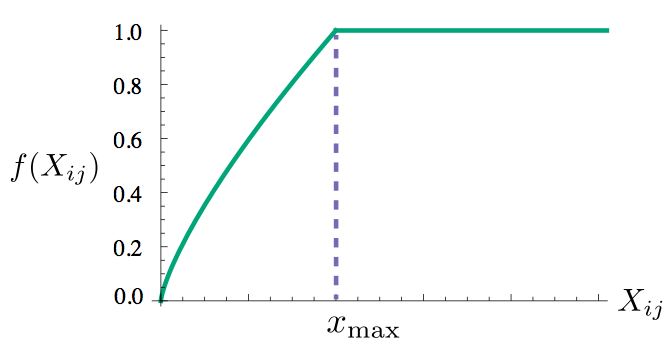
\includegraphics[scale=0.27]{images/weighting.png}
      \caption{From}
    \end{figure}
\end{frame}

%%%%%%%%%%%%%%%%%%%%%%%%%%%%%%%%%%%%%%%%%%%%%%%%%%
%% \begin{frame}{Training}
  %% \begin{itemize}
  %% \item Vector Length:
  %% \item Context Size: 
  %% \item Corpus Size: nothing supriszing
  %% \end{itemize}
%% \end{frame}

%%%%%%%%%%%%%%%%%%%%%%%%%%%%%%%%%%%%%%%%%%%%%%%%%%
\begin{frame}{Model Analysis}
  \begin{itemize}
  \item Vector Length:
  \item Context Size: 
  \item Corpus Size: nothing suprising
  \end{itemize}
\end{frame}

%%%%%%%%%%%%%%%%%%%%%%%%%%%%%%%%%%%%%%%%%%%%%%%%%%
\begin{frame}{Results}
    \begin{figure}
      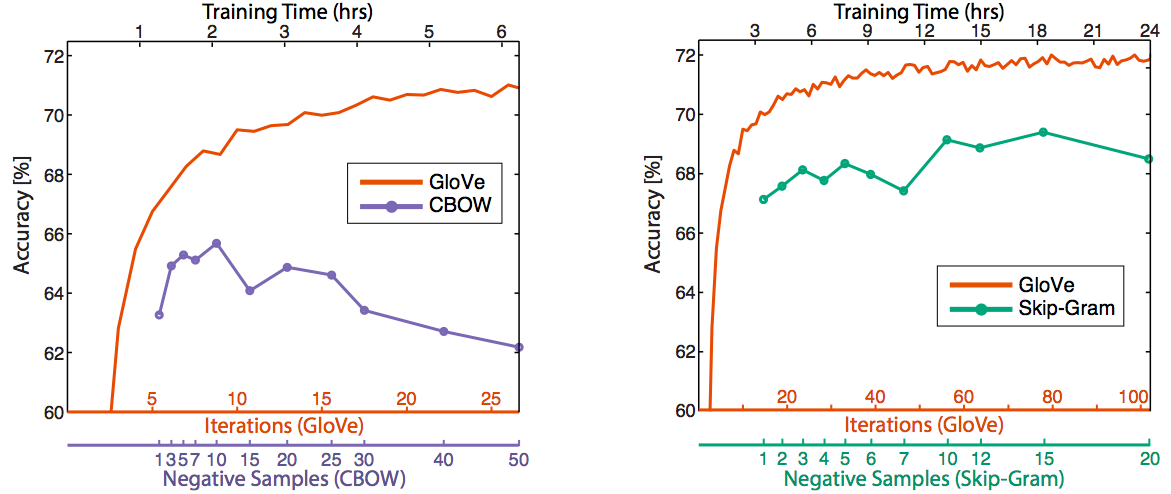
\includegraphics[scale=0.27]{images/gloveVSword2vec.png}
      \caption{From}
    \end{figure}
\end{frame}

%%%%%%%%%%%%%%%%%%%%%%%%%%%%%%%%%%%%%%%%%%%%%%%%%%
\begin{frame}{Results}
  \begin{figure}
    \centering
    \begin{subfigure}[b]{0.33\textwidth}
      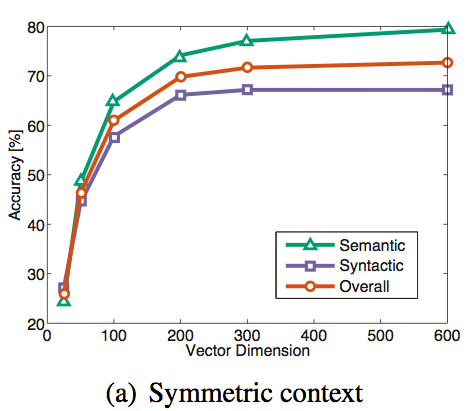
\includegraphics[width=\textwidth]{images/analogy1.png}
    \end{subfigure}%
    \begin{subfigure}[b]{0.33\textwidth}
      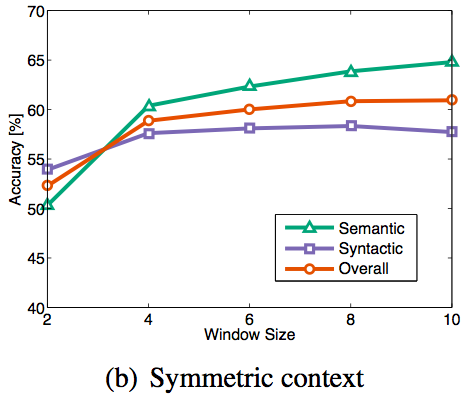
\includegraphics[width=\textwidth]{images/analogy2.png}
    \end{subfigure}%
    \begin{subfigure}[b]{0.33\textwidth}
      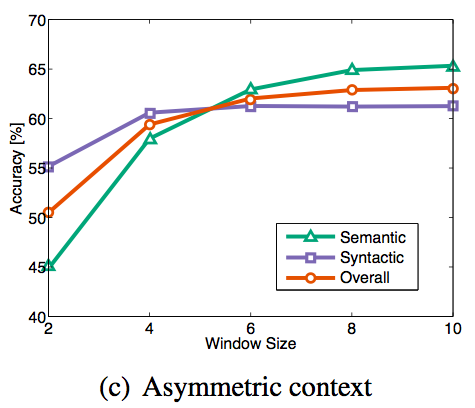
\includegraphics[width=\textwidth]{images/analogy3.png}
    \end{subfigure}%
  \end{figure}
\end{frame}
